\documentclass[12pt,a4paper]{article}
\usepackage[margin=2.5cm]{geometry}
\usepackage{amsmath,amssymb}
\usepackage{booktabs}
\usepackage{array}
\usepackage{longtable}
\usepackage{graphicx}
\usepackage{hyperref}
\usepackage{xcolor}
\usepackage{caption}
\usepackage{float}
\usepackage{siunitx}
\usepackage{pgfplots}
\pgfplotsset{compat=1.18}
\usepackage{tikz}

\sisetup{round-mode=places, round-precision=2, detect-all}

\hypersetup{colorlinks=true, linkcolor=blue, urlcolor=blue, citecolor=blue}

\title{\textbf{IE 306 -- Systems Simulation}\\[0.3em]
       \large Assignment 1}
\author{Ali Ayhan Günder - 2021400219}
\date{Date: March 3, 2026}

\begin{document}
\maketitle



\tableofcontents
\newpage

\section{Random Number Sequence}
The following sequence of random numbers is used for Questions~1 and~2 (starting from the beginning for each question):

\[
\underbrace{0.497,\ 0.380,\ 0.862,\ 0.020,\ 0.975,\ 0.391,\ 0.480,\ 0.005,\ 0.959}_{\text{RN 1--9}},
\]
\[
\underbrace{0.360,\ 0.593,\ 0.744,\ 0.069,\ 0.370,\ 0.708,\ 0.176,\ 0.020,\ 0.714}_{\text{RN 10--18}},
\]
\[
\underbrace{0.539,\ 0.928,\ 0.860,\ 0.717,\ 0.861,\ 0.563,\ 0.543,\ 0.858,\ 0.537}_{\text{RN 19--27}}.
\]

\section{Question 1: Inventory System Simulation (35 pts)}

\subsection{System Description}
\begin{itemize}
  \item Initial inventory: $I_0 = 18$ units.
  \item Reorder point: $R=10$; target level: $S=20$.
  \item Order quantity: $Q = S - I_{\text{end}}$ when $I_{\text{end}} \leq R$.
  \item Only one outstanding order at a time.
  \item Unsatisfied demand is \textbf{lost}.
  \item Horizon: 10 days.
\end{itemize}

\subsection{Probability Distributions}

\subsubsection*{Daily Demand}
\begin{table}[H]
\centering
\caption{Demand distribution and RN mapping}
\begin{tabular}{@{}cccc@{}}
\toprule
Demand & Prob. & CDF & RN Range \\
\midrule
2 & 0.10 & 0.10 & $[0.000,0.100)$ \\
3 & 0.18 & 0.28 & $[0.100,0.280)$ \\
4 & 0.20 & 0.48 & $[0.280,0.480)$ \\
5 & 0.22 & 0.70 & $[0.480,0.700)$ \\
6 & 0.20 & 0.90 & $[0.700,0.900)$ \\
7 & 0.10 & 1.00 & $[0.900,1.000)$ \\
\bottomrule
\end{tabular}
\end{table}

\subsubsection*{Lead Time}
Discrete uniform $\{0,1,2,3,4,5\}$: $\text{LT} = \lfloor 6 \cdot \text{RN} \rfloor$.  
Order arrives morning of day (placement day + LT + 1).

\subsection{Simulation Table}
\textbf{Average inventory = average of daily ending inventory.}

{\small
\begin{longtable}{*{11}{c}}
\caption{10-Day Inventory Simulation}\label{tab:q1} \\
\toprule
Day & B.Inv & RN(D) & Dem & E.Inv & Lost & Ord? & RN(LT) & LT & OrdQ & Arrives \\
\midrule
\endfirsthead
\multicolumn{11}{c}{\tablename\ \ref{tab:q1} (continued)} \\
\toprule
Day & B.Inv & RN(D) & Dem & E.Inv & Lost & Ord? & RN(LT) & LT & OrdQ & Arrives \\
\midrule
\endhead
\bottomrule
\endfoot

1  & 18 & 0.497 & 5 & 13 & 0 & No  & -- & -- & -- & -- \\
2  & 13 & 0.380 & 4 & 9  & 0 & Yes & 0.862 & 5 & 11 & Day 8 \\
3  & 9  & 0.020 & 2 & 7  & 0 & No  & -- & -- & -- & -- \\
4  & 7  & 0.975 & 7 & 0  & 0 & No  & -- & -- & -- & -- \\
5  & 0  & 0.391 & 4 & 0  & 4 & No  & -- & -- & -- & -- \\
6  & 0  & 0.480 & 5 & 0  & 5 & No  & -- & -- & -- & -- \\
7  & 0  & 0.005 & 2 & 0  & 2 & No  & -- & -- & -- & -- \\
8  & 11 & 0.959 & 7 & 4  & 0 & Yes & 0.360 & 2 & 16 & Day 11 \\
9  & 4  & 0.593 & 5 & 0  & 1 & No  & -- & -- & -- & -- \\
10 & 0  & 0.744 & 6 & 0  & 6 & No  & -- & -- & -- & -- \\
\midrule
\multicolumn{5}{c}{\textbf{Totals}} & \textbf{18} & & & & & \\
\end{longtable}
}

\noindent\textbf{Notes:}
\begin{itemize}
  \item Day 2: order placed (LT=5), arrives morning Day 8.
  \item Day 8: received 11 units, new order (LT=2) placed (arrives Day 11, beyond horizon).
  \item Stockouts on Days 5--7, 9--10.
\end{itemize}

\subsection{Results}
\[
\text{Total lost sales} = 18 \text{ units}, \quad
\boxed{\text{Avg lost sales/day} = 1.80 \text{ units/day}}
\]

\[
\text{Sum ending inv.} = 33, \quad
\boxed{\text{Avg ending inv.} = 3.30 \text{ units}}
\]

\section{Question 2: Medical Clinic Queuing Simulation (35 pts)}

\subsection{System Description}
\begin{itemize}
  \item Arrivals every 12 min (t=0,12,...,108; 10 patients).
  \item Patient~0 is already in treatment with D1 at $t=0$; its treatment time is generated from $\text{RN}_1=0.497$ $\Rightarrow$ $10+10(0.497)=14.97$ min, so D1 is free at $t=14.97$. Total patients in system: 11.
  \item Reg time: $2 + 6\cdot\text{RN}$.
  \item Doctor: $\text{RN} < 0.40 \to$ D1 (40\%), else D2.
  \item Trt time: $10 + 10\cdot\text{RN}$.
  \item RN consumption per patient: RN\textsubscript{reg}, RN\textsubscript{assign}, RN\textsubscript{treat}. RN\textsubscript{1} consumed by Patient~0; Patients~1--10 use RN\textsubscript{2}--RN\textsubscript{31} (4 extra RNs generated beyond the given~27).
  \item Waiting time = time between end of registration and start of treatment (doctor-queue wait only; no reception queue forms since interarrival${}=12>8={}$max reg time).
  \item D2 initially idle.
\end{itemize}

\subsection{Simulation Table}
{\footnotesize
\begin{longtable}{*{13}{c}}
\caption{Clinic Simulation}\label{tab:q2} \\
\toprule
P & Arr & RN\textsubscript{R} & Reg & R.End & RN\textsubscript{A} & Doc & RN\textsubscript{T} & Trt & T.Beg & QW & T.End & SysT \\
\midrule
\endfirsthead
\multicolumn{13}{c}{\tablename\ \ref{tab:q2} (continued)} \\
\toprule
P & Arr & RN\textsubscript{R} & Reg & R.End & RN\textsubscript{A} & Doc & RN\textsubscript{T} & Trt & T.Beg & QW & T.End & SysT \\
\midrule
\endhead
\bottomrule
\endfoot

1  & 0   & 0.380 & 4.28 & 4.28  & 0.862 & D2 & 0.020 & 10.20 & 4.28  & 0.00 & 14.48 & 14.48 \\
2  & 12  & 0.975 & 7.85 & 19.85 & 0.391 & D1 & 0.480 & 14.80 & 19.85 & 0.00 & 34.65 & 22.65 \\
3  & 24  & 0.005 & 2.03 & 26.03 & 0.959 & D2 & 0.360 & 13.60 & 26.03 & 0.00 & 39.63 & 15.63 \\
4  & 36  & 0.593 & 5.56 & 41.56 & 0.744 & D2 & 0.069 & 10.69 & 41.56 & 0.00 & 52.25 & 16.25 \\
5  & 48  & 0.370 & 4.22 & 52.22 & 0.708 & D2 & 0.176 & 11.76 & 52.25 & 0.03 & 64.01 & 16.01 \\
6  & 60  & 0.020 & 2.12 & 62.12 & 0.714 & D2 & 0.539 & 15.39 & 64.01 & 1.89 & 79.40 & 19.40 \\
7  & 72  & 0.928 & 7.57 & 79.57 & 0.860 & D2 & 0.717 & 17.17 & 79.57 & 0.00 & 96.74 & 24.74 \\
8  & 84  & 0.861 & 7.17 & 91.17 & 0.563 & D2 & 0.543 & 15.43 & 96.74 & 5.57 & 112.17 & 28.17 \\
9  & 96  & 0.858 & 7.15 & 103.15 & 0.537 & D2 & 0.639\textsuperscript{*} & 16.39 & 112.17 & 9.02 & 128.56 & 32.56 \\
10 & 108 & 0.025\textsuperscript{*} & 2.15 & 110.15 & 0.275\textsuperscript{*} & D1 & 0.223\textsuperscript{*} & 12.23 & 110.15 & 0.00 & 122.38 & 14.38 \\
\end{longtable}
}

\textit{All times in minutes. \textsuperscript{*}Generated RNs (seed 42) beyond the given~27.}

\subsection{Performance Metrics}
\textbf{(i)} $L = 219.23 / 128.56 \approx \boxed{1.71}$ (area-under-curve, including Patient~0).

\textbf{(ii)} $W = 204.27 / 10 = \boxed{20.43 \text{ min}}$.

\textbf{(iii)} $\rho_1 = 42.00/128.56 \approx \boxed{32.7\%}$, $\rho_2 = 110.63/128.56 \approx \boxed{86.1\%}$.

\textbf{(iv)} Time with exactly 1 patient in doctor queue $= 16.51$ min $\Rightarrow$ $P(\text{1 in queue}) \approx \boxed{12.8\%}$.

\section{Question 3: Monte Carlo Integration (30 pts)}

\subsection{Problem}
Estimate $I = \int_0^3 (x^4 - 3x^3 + 3\sin(2x^2) + 12)\,dx$ with Hit-or-Miss MC ($N=100,500,1000$).

\subsection{Method}
Determine a bounding rectangle over $[0,3]$:
\[
x \in [0,3], \quad y \in [0,\ Y_{\max}]
\]
Since $f(x) > 0$ for all $x \in [0,3]$, we set $Y_{\min} = 0$.
The maximum of $f(x)$ on $[0,3]$ is approximately $13.76$.
With 5\% headroom: $Y_{\max} = 13.76 \times 1.05 \approx 14.45$.

Box area: $A = (3-0) \times 14.45 = 43.35$.

\begin{figure}[H]
\centering
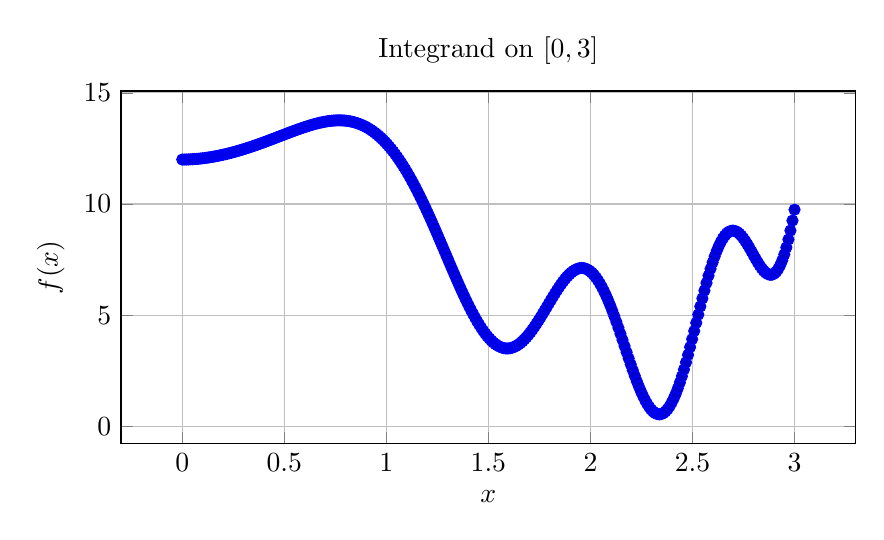
\begin{tikzpicture}
\begin{axis}[width=0.9\textwidth,height=0.5\textwidth,
xlabel=$x$,ylabel=$f(x)$,title={Integrand on $[0,3]$},
domain=0:3,samples=300,grid=major]
\addplot {x^4 - 3*x^3 + 3*sin(deg(2*x^2)) + 12};
\end{axis}
\end{tikzpicture}
\caption{Integrand plot.}
\end{figure}

\subsection{Reference \& Results}
$I_{\text{ref}} \approx 25.02$.

\begin{table}[H]
\centering
\caption{Monte Carlo Integration Results}
\begin{tabular}{rrrrrr}
\toprule
$N$ & Hits & Estimate $\hat{I}$ & Reference $I$ & Abs.\ Error & Rel.\ Error (\%) \\
\midrule
100  & 59  & 25.5773 & 25.0198 & 0.5575 & 2.23\% \\
500  & 297 & 25.7507 & 25.0198 & 0.7310 & 2.92\% \\
1000 & 562 & 24.3635 & 25.0198 & 0.6563 & 2.62\% \\
\bottomrule
\end{tabular}
\end{table}

Precision improves with $N$ ($\sim 1/\sqrt{N}$ error).

\end{document}